\documentclass{article}
\usepackage[utf8]{inputenc}
\usepackage{graphicx}
\usepackage{amssymb, amsmath, amsthm}
\usepackage{bbm}
\usepackage{biblatex}
\usepackage{floatrow}
\newfloatcommand{capbtabbox}{table}[][\FBwidth]
\addbibresource{references.bib}
\newcommand\numberthis{\addtocounter{equation}{1}\tag{\theequation}}
\usepackage[margin=1in]{geometry}
\graphicspath{ {report_figures/} }
\parskip = 0.1in

\begin{document}
\title{Forest Fires: An Analysis of the Initial Spread Index}
\author{Nate Josephs\footnote{Introduction, Feature Design, Variable Selection, Appendix, Discussion} Matthew Wiens\footnote{Feature Design, Variable Selection, Prediction, Discussion} Aaron Elliot\footnote{Modeling, Bootstrapping, Background, Discussion} Kelly Kung\footnote{Modeling, Data Transformations, Data Overview, Discussion} Ben Draves\footnote{Modeling, Variable Selection, Bootstrapping, Appendix, Discussion}}
\date{December 12, 2017}
\maketitle
\begin{abstract}
Forest fires continue to be a serious ecological issue that endanger human lives and ravage environmental systems. At the time of this report, devastating wild fires are sweeping through Southern California and have destroyed more than 5,700 structures with more than 3,000 acres of land still burning. While human ability to fight forest fires has improved dramatically over recent decades, prevention is still the most effective course to minimizing environmental damage. The \textit{Initial Spread Index (ISI)} is a metric that quantifies the speed at which a fire spreads. Firefighting agencies can use this metric to issue public warnings and deploy resources to most effectively monitor and contain forest fires before they cause substantial harm. This analysis uses linear modeling methodologies to infer key components that affect $\textit{ISI}$ and by extension determine what causes rapid spread of forest fires. Through penalization schemes and iterative model construction, we find that \textit{wind speed}, \textit{temperature}, and a \textit{summer indicator variable} all significantly explained \textit{ISI}. With this result, firefighting groups can leverage existing weather prediction systems to more effectively monitor and detect threats of deadly forest fires.
\end{abstract}

\section{Introduction}
Forest fires demolish entire ecosystems and have lasting consequences on the environment beyond their path of destruction. These fires deplete oxygen from the atmosphere, impact the lumber industry, vanquish animal habitats, and damage areas of natural beauty. They also contribute to pollution, carbon emission, soil erosion, flooding, and water contamination. As our planet is increasingly threatened by rising temperatures and dangerous policies, it is imperative that we be more responsible with our resources. Statistics offers many tools that can reveal ways to be more mindful and efficient in addressing complex problems. Here, we will use the theory of linear modeling to analyze the initial spread of forest fires. In particular, we look to pick up where Smokey Bear left-off: the next line of defense after prevention is early-detection. By understanding the factors of initial spread, we hope to contribute to the fight against forest fires.

To accomplish this goal, we examine \textit{Initial Spread Index (ISI)} as our response variable from data obtained in Monteshino Natural Park between 2000 and 2003. It is worth emphasizing that our target is not forest fire occurrences. This subtle difference goes against our intuition. For example, regarding people, we expect that the number of fires increases with the presence of people. On the other hand, more people means earlier detection. Therefore, we have no $\textit{a priori}$  knowledge of the relationship between people and \textit{ISI}. This difficulty extends to other variables such as rain and wind, in which different arguments could be made to explain different possible relationship with \textit{ISI}.

This paper is organized as follows. In Section \ref{Background} we give a summary of our reference paper and restate our goal in this context. In Section \ref{Analysis} we outline our analysis, including our initial exploration of the data, all feature engineering and variable selection, and our final modeling decisions. In Section \ref{Prediction}, we apply our final model to our holdout set in order to make unbiased inferences. We conclude our project in Section \ref{Discussion} with a general discussion of our results and possible future directions. Finally, R code for inline plots and the final modeling process may be found in Appendix I and Appendix II, respectively.

\section{Background}\label{Background}

%The subject of modeling forest fires has been well studied.
In the reference paper provided\footnote{P. Cortez and A. Morais. A Data Mining Approach to Predict Forest Fires using Meteorological Data. In J. Neves, M. F. Santos and J. Machado Eds., New Trends in Artificial Intelligence, Proceedings of the 13th EPIA 2007 - Portuguese Conference on Artificial Intelligence, December, Guimares, Portugal, pp. 512-523, 2007.}, Cortez and Morais explored the potential of machine learning algorithms for predicting area burned by forest fires. They compared support vector machines (SVM), decision trees, multiple linear regression, neural networks, random forests, and a na\"ive mean prediction with four sets of features. The authors found that SVMs had the overall best success in predicting area burned using a combination of $\textit{temperature}$, $\textit{rain}$, $\textit{relative humidity}$ and $\textit{wind speed}$. Furthermore, their analysis details that in the Fire Weather Index (FWI) system, $\textit{ISI}$ is a complex function of $\textit{wind}$ and $\textit{Fire Fuel Moisture Code (FFMC)}$. We incorporate this discovery in our own analysis.

We use the same data curated by Cortez and Moraid, which includes meteorological data, as well as burned areas of forest fires within Montesinho Natural Park in the northeast Tr\'as-os-Montes region of Portugal. The data were collected from January 2000 to December 2003 in separate datasets, which were manually integrated by the authors into a single dataset with a total of 517 observations. It should be noted that Cortez and Moraid do not claim this is a totally comprehensive dataset; some of the forest fires in the area may not have been recorded. We keep this in mind with regard to possible sampling bias.

Our analysis takes a standard approach by first splitting the data into training and testing sets (70-30\% split), then performing feature engineering and variable selection on our training set, fitting our various models, and finally evaluating these models on our testing set. We acknowledge that due to the relatively small sample size of the dataset, there may be sparsity concerns in our training and testing sets. We address these issues as they arise. While we do make predictions on the test set, our focus is on making statistically significant inferential conclusions. Therefore, we avoid using overly complicated transformations, and when faced with competing models, we select the simpler version. We understand that this may result in a sub-optimal predictive model, but our goal is to obtain interpretable coefficients and generalizable results. We chose this inferential approach because we believe the first step to combating forest fires is understanding how they initially spread, and without an understanding, what good is a highly predictive model? Naturally we want to understand the likely causes of forest fires with a high $\textit{ISI}$, of which we explore variables related to weather, time, location, and people.

\section{Modeling \& Analysis}\label{Analysis}

\subsection{Data Overview}\label{data_over}

The \textit{ISI} attempts to quantify the risk associated with the initial spread of a forest fire. Heuristically, we expect variables that describe the weather characteristics of Monteshino Natural Park, as well as the terrain within the park, to affect the initial spread of a newly sparked forest fire. Although we do not know exactly how $\textit{ISI}$ is calculated, we surmise that these characteristics should play a major role in our modeling procedure. While we expect weather and human impact to be two major explanatory classes, there is a third, far more subtle factor that we need to address. Consider Figure \ref{fig:human_factor}. 
\begin{figure}[h!]
\centering
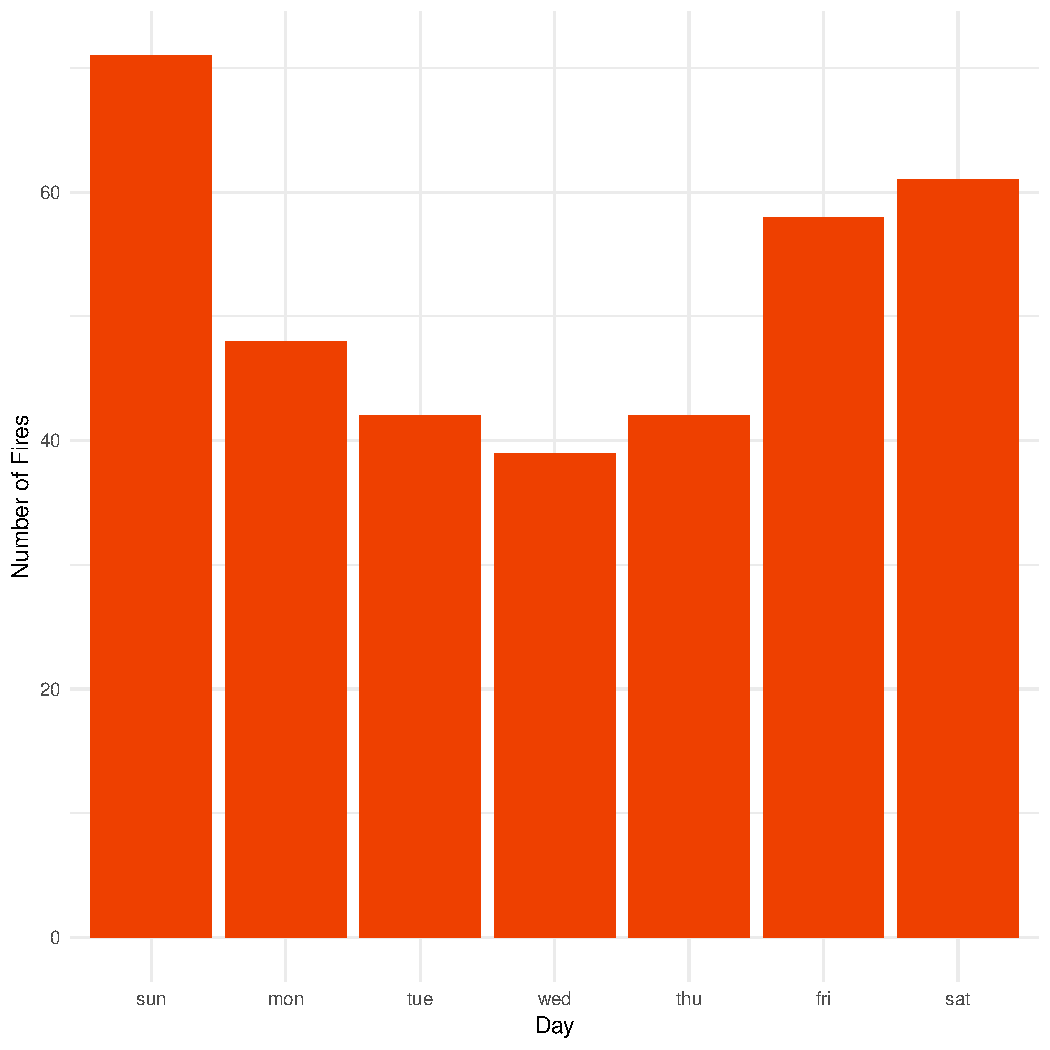
\includegraphics[scale = .25]{day_bar.pdf}
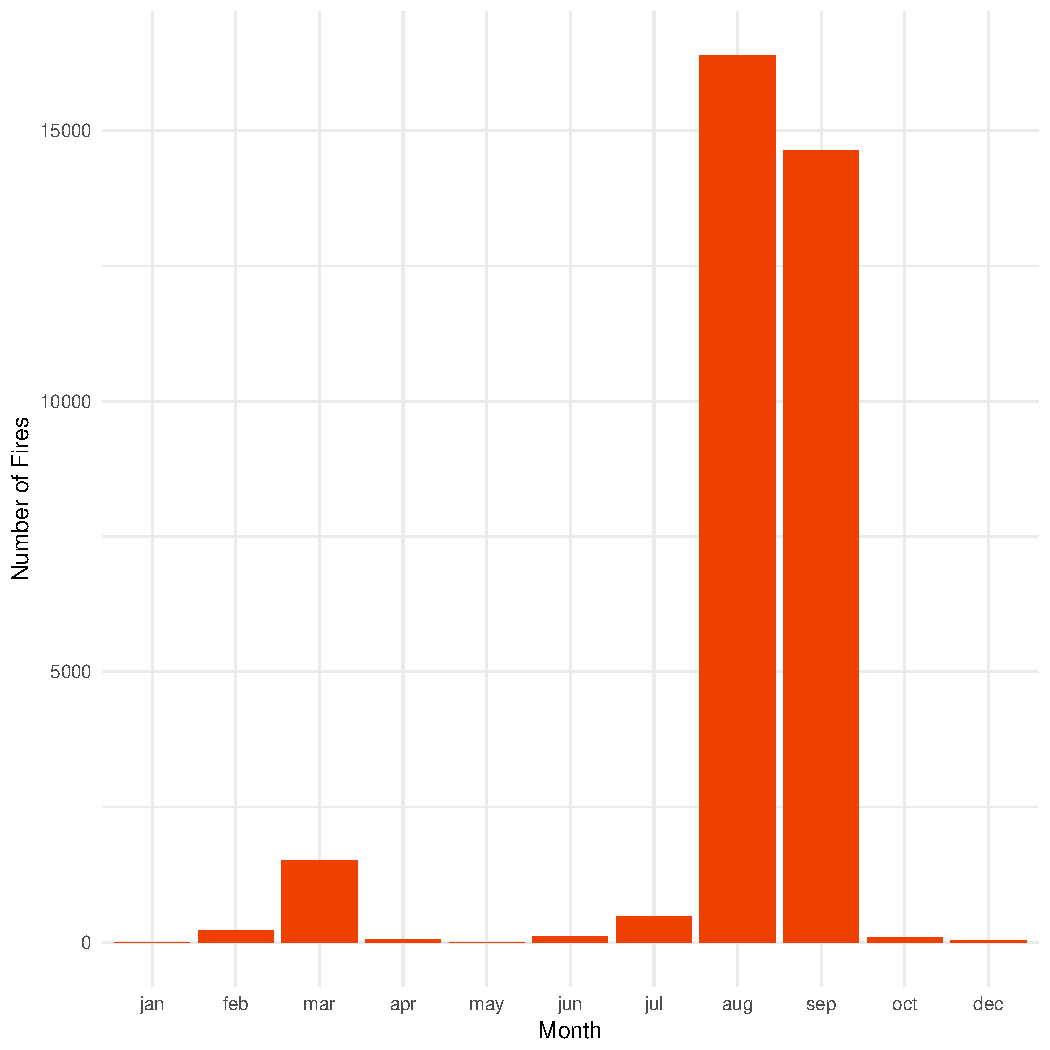
\includegraphics[scale = .25]{month_bar.pdf}
\caption{The data suggest more fires occur on the weekend and during the summer months.}
\label{fig:human_factor}{}
\end{figure}
It appears that fires are far more likely to occur in late summer and on the weekends. While the abundance of fires occurring in summer may be attributable to weather patterns\footnote{With a large spike in March, however, this behavior could be explained by both human behavior and weather trends.}, we suspect that the imbalance of fires on the weekend is connected in some way to the presence of more visitors to the park. Although we do not have direct data on the number of individuals in the park on any given day, we expect that this variable greatly affects the way in which \textit{the data were collected}. It seems reasonable to assume park visitors were either responsible for reporting the presence of a fire or starting the fires themselves. Therefore, when more visitors are in the park, we expect more fires to be detected, and more observations to be included in our dataset. So although we expect visitors to have no affect on how fast fires spread, due to the nature in which the data were collected, we include variables that model human presence.  

With this in mind, we categorize our data into four types: weather, FWI indices, geo-spatial, and human impact. Weather covariates include rain totals, temperature, and relative humidity, while indices such as \textit{FFMC}, \textit{Duff Moisture Code (DMC)}, and \textit{Drought Code (DC)} attempt to measure characteristics of the terrain. We attempt to capture the effect of geo-spatial components by using the $(X,Y)$ coordinates, as well as designing new variables that identify homogeneous regions of the park. Lastly, we model the human impact inherent in data collection by introducing variables that serve as proxies for the number of visitors to the park on any given day. The construction of these variables will be covered in detail in Section \ref{Engineering}.

In addition to these features, we also note that during our modeling procedure we found two abnormal instances of the response, \textit{ISI}, in our training set: one point had a value of zero and another had a value 56.1. Considering the boxplot in Figure \ref{fig:ISI_outlier},
\begin{figure}[h!]
\centering
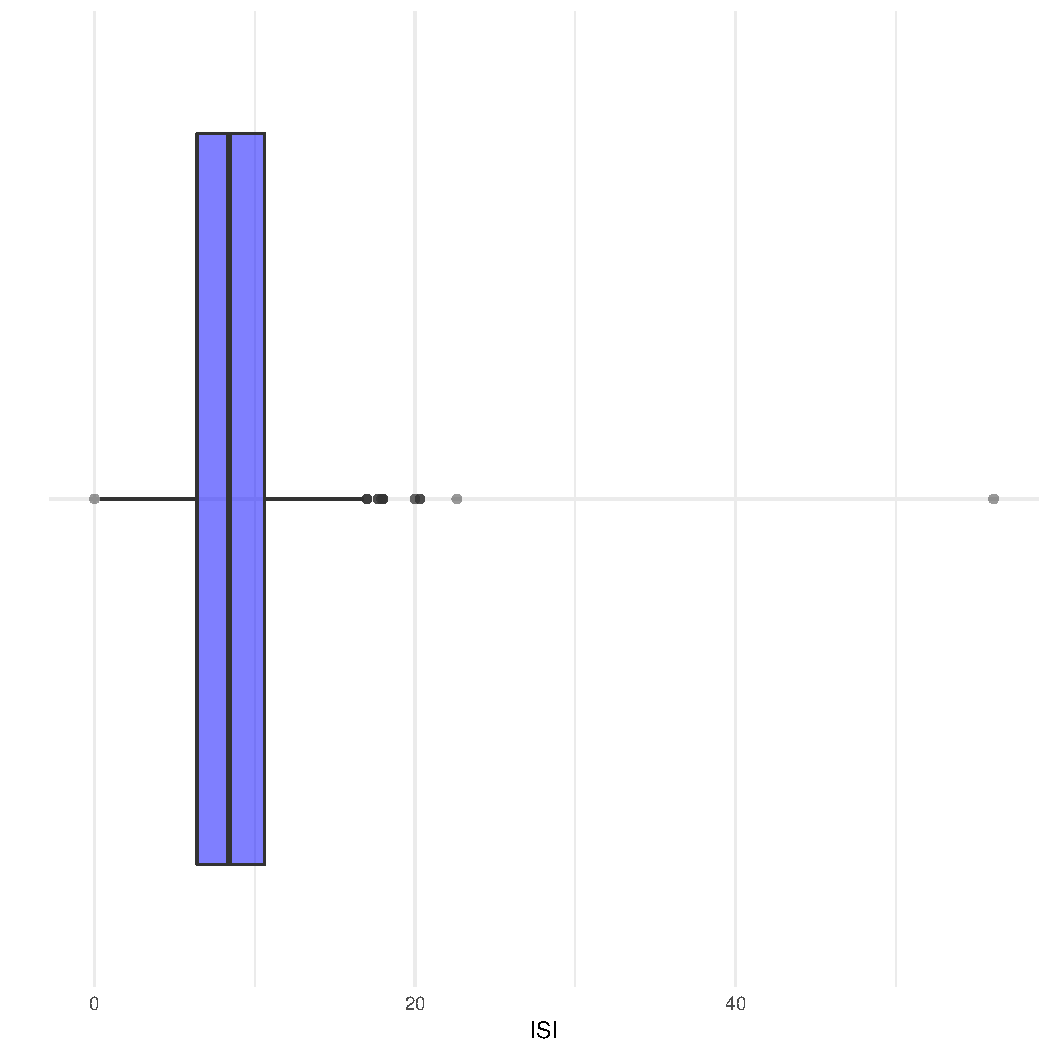
\includegraphics[width = .5\textwidth, height = 4cm]{ISI_box.pdf}
\caption{The boxplot of $ISI$ suggests that there are significant outliers in our data.}
\label{fig:ISI_outlier}{}
\end{figure}
these two points, especially the outlier for $\textit{ISI} = 56.1$, should be investigated. Upon further analysis, we were unable to identify any specific reason that these values deviated so far from the mean of the distribution. For this reason, we do not remove them from the training set. Instead, we performed sensitivity analysis during each step of the modeling process by repeating our analysis with and without these points, and concluded that the analysis was similar in both cases. Henceforth, we present only our results with these outliers included.

\subsection{Feature Design}\label{Engineering}

Based on our intuition of \textit{ISI}, as well as an initial look at the data, we transformed and created several covariates to obtain more informative predictors. We first found that area burned \textit{(area)} is highly concentrated around zero\footnote{Any fire with burn area lower than $100m^2$ was considered zero.} and extremely right skewed. Following the analysis of Cortex and Morais, we transformed $\textit{area}$ using $\textit{areaTrans} = \ln(\textit{area} + 1)$. The rain fall \textit{(rain)} covariate is also concentrated around zero and right skewed, but we note that only 1.7\% of the training set was non-zero. Therefore, we created an indicator of whether or not there was rain on the day of the given fire $(\textit{rainvnorain})$. 

In order to better support our intuition about the impact of weather on $\textit{ISI}$, we also created a wetness metric, \textit{wetness}, that measures the moisture in the air. We expect that this variable is important, because if there is more moisture in the air, then fires should not be able to spread as easily. Furthermore, if there is more moisture in the air, then plants and trees are also more moist, which means that fires lack the dry fuel they need in order to spread. To calculate this metric, we obtained initial values of \textit{wetness} using the LennTech calculator\footnote{https://www.lenntech.com/calculators/humidity/relative-humidity.htm} by identifying wetness values for corresponding temperature $(\textit{temp})$ and relative humidity $(\textit{RH})$ values. We then approximate this function in order to obtain metric values for each observation in our dataset. 

We also created new indicators for the human impact feature class based on our initial analysis as explained in Section \ref{data_over}. We created the indicators \textit{summer} and \textit{weekend}, because we observed that more fires occurred during these time periods. In particular, $\textit{summer} = 1$ corresponds to the months of \textit{June, July, August}, and \textit{ September}. These months were chosen based on the climate of Portugal and the number of fires that occurred in this time frame. As for \textit{weekend}, we chose the standard weekend days, $\textit{Friday, Saturday,}$ and $\textit{Sunday}$, to receive a 1.

Another interesting feature class in this problem is geo-spatial. The raw data contains $X$ and $Y$ coordinates corresponding to a grid that has been overlaid on the map of Monteshino Natural Park. Each coordinate ranges from 1 to 9, therefore there are 81 total boxes in the grid. Of course, the first attempts at capturing any geo-spatial signal involved looking at the raw $X$ and $Y$ coordinates, as well as their interaction. Unfortunately, many of these boxes were sparse and the 81 degrees of freedom necessary for the raw grid were detrimental to the modeling process. Instead, we designed several features based on these values. This resulted in three candidate features. First, we created new coordinates $X2$ and $Y2$ that were created from the following algorithm
\begin{align*}
1&. \text{ Set } X2 = X \text{ and } Y2 = Y. \\
2&. \text{ Sum the first row, last row, first column, and last column of the } X2-Y2 \text{ matrix.} \\
3&. \text{ Combine the row or column with the lowest sum with its neighboring row or column.} \\
4&. \text{ Repeat steps 2 and 3 until every entry contains at least 1\% of the data.}
\end{align*}
The algorithm was written under the belief that neighboring spaces should be topographically similar and therefore should be the first candidates when grouping spaces together. Applying this algorithm, we reduced the number of boxes from 81 to 12. We note that $Y2$ only has two levels, which is unsurprising since Monteshino Natural Park is wider than it is tall. The other two engineered features integrated outside information. For these, we found a topographical map of Monteshino Natural Park on Google Maps and overlaid the original $X-Y$ grid.  The result may be found in Appendix II. From this, we created \textit{forest\_ind}, which is a binary variable that takes the value 1 when the box is mostly covered in trees and 0 otherwise, and \textit{grid\_group}, which identifies five major mountain ranges and groups the boxes that cluster around these mountain ranges. Both of these variables are intuitively appealing, since forest fires burn more rapidly when trees are nearby and generally hikers tend to favor certain mountain ranges, which may have an effect on how fires are started. 

Lastly, we used a Box-Cox Transformation to identify the appropriate power transformation for our response variable. The result was $\lambda = \frac{1}{2}$, corresponding to a square-root transformation, yielding our new response variable \textit{sqISI}. Since $\textit{ISI}$ is an index, it is unitless. Therefore, we feel comfortable transforming it without loss of interpretation.

\subsection{Variable Selection}\label{Var_Sel}

In order to effectively consider all variables discussed above (along with several interaction terms), while still making inferential statements about \textit{sqISI}, we use penalization schemes in order to identify important variables and classes of variables in our problem.\footnote{While we considered forward and backwards model selection procedures, information-theoretic approaches typically require normally-distributed residuals, which we found to be an unreasonable assumption based on our initial fits.} While Ridge Regression has several nice properties, we utilize LASSO for its ability to perform variable selection. By using LASSO, we allow an $L_{1}$ penalty to \textit{zero-out} non-informative variables while also identifying variables that are representative of entire classes of covariates, e.g weather, spatial, etc.

After considering penalization coefficients under optimal smoothing parameters, as well as the added variable plots in successive iterations of the modeling procedure, we found that a model including the variables \textit{summer}, \textit{temp}, and \textit{FFMC} were all key components in the mean function of $\textit{sqISI}$. We note that the three engineered geo-spatial features from Section \ref{Engineering} were all considered as covariates, but unfortunately none were selected, as either LASSO zeroed-out their coefficients or they were deemed not significant under further scrutiny. Since we still expect that terrain should play a role in describing \textit{sqISI}, we attempted to include this information in more complex ways in Section \ref{candidate}. On the other hand, representatives of weather, human impact, and FWI indices were all included. Lastly we note that all interaction terms were also zeroed-out by LASSO.  

With these covariates, we fit a linear regression model to the data and find that this model performed very poorly. The residuals appears highly non-normal with non-constant variance. In addition, it appeared that any covariate except \textit{FFMC} played little role in the model. Investigating the bivariate plot of \textit{sqISI} and \textit{FFMC}, found in Figure \ref{fig:FFMC_ISI_scatter}, we see that \textit{FFMC} and \textit{sqISI} are almost perfectly related, but in a non-linear fashion.  
\begin{figure}[h!]
\centering
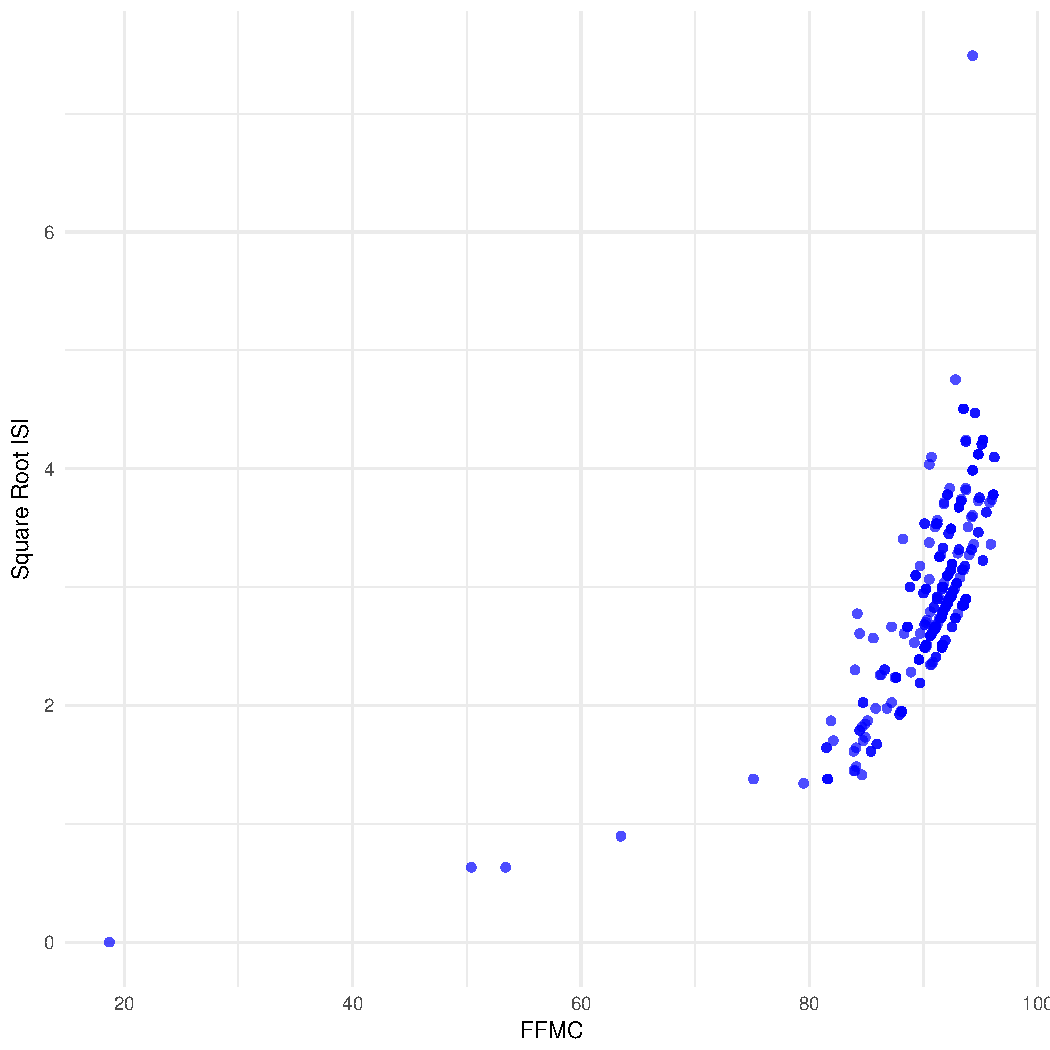
\includegraphics[scale = 0.4]{FFMC_ISI_scatter.pdf}
\caption{While \textit{FFMC} and \textit{sqISI} are closely related, this relationships is nonlinear.}
\label{fig:FFMC_ISI_scatter}
\end{figure}
Seeing the tight association between these two variables, it follows that any model selection procedure will rightfully include \textit{FFMC} as a predictor. But due to the non-linearity inherent in this plot, any model including \textit{FFMC} fails to satisfy the linear modeling assumptions. Now, if our goal is prediction, then we would simply fit a higher order polynomial of \textit{FFMC}, which would successfully explain the majority of the variance in \textit{sqISI}. This approach, however, would only reveal the relationship between \textit{sqISI} and \textit{FFMC}. Also, we know from Cortez and Morais that \textit{FFMC} is a function of the other covariates found in this model (e.g. \textit{wind}, \textit{temp}, etc.). Therefore, we would only be able to infer the dependence between these other covariates and \textit{sqISI} \textit{through FFMC}. In this way, \textit{FFMC} effectively masks the explanatory value of the other covariates. To illustrate this, consider the penalization paths with and without $\textit{FFMC}$ in Figure \ref{fig:pen_plots}.
\begin{figure}[h!]
\centering
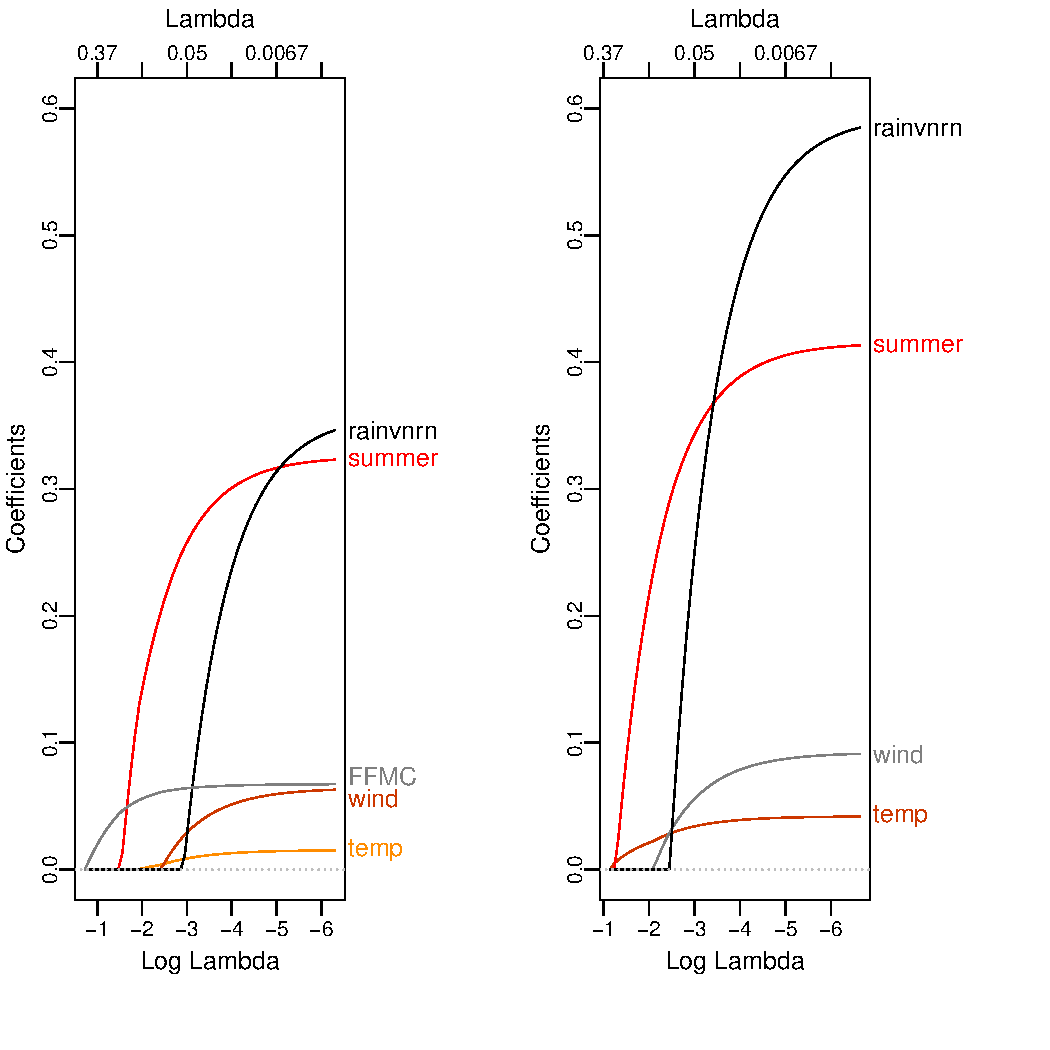
\includegraphics[scale = .4]{penalization_plots.pdf}
\caption{Removing \textit{FFMC} from our modeling procedure suggests that \textit{FFMC} and the weather covariates explain similar variability in \textit{sqISI}.}
\label{fig:pen_plots}{}
\end{figure}
Notice how when we exclude \textit{FFMC}, the other variables' relative importance grows, while their penalization paths maintain a similar shape. Therefore, we see that $\textit{FFMC}$ and this set of covariates do, in fact, model similar variability in \textit{sqISI}. This was not immediately obvious by looking at correlation values and other collinearity statistics due to the non-linear relationship between \textit{FFMC} and \textit{sqISI}, but by investigating their penalization paths, we see that \textit{FFMC} is skewing our analysis. 

Since we chose an inferential approach to this problem, we wish to see the direct relationship between \textit{sqISI}, and hence $\textit{ISI}$, and the other covariates considered above. Therefore, we wish to simplify the \textit{FFMC} variable and use the information from this variable in a way that does not mask the effects of \textit{wind}, \textit{summer}, \textit{rainvnorain}, and \textit{temp}. While we tried several different transformations of \textit{FFMC} to make this pairwise relationship linear, we could find no interpretable function that resolved this issue. Instead, we note that this complex non-linear relationship is roughly piecewise linear around the point $FFMC = 80$. Therefore, we introduce an indicator variable $\textit{(tFFMC)}$ for $FFMC\leq 80$ into our modeling procedure.

After introducing $tFFMC$ into the modeling procedure, our final penalized coefficient estimates after iterative variable selection are given in Table 1. 
\begin{figure}[h!]
\begin{floatrow}
\capbtabbox{%
\begin{tabular}{l|c||l|c}{}
Variable & $|\beta|$ & Variable & $|\beta|$\\
\hline
\hline
tFFMC & 1.51 & X2:7 & 0.07 \\
rainvnorain & 0.66 & temp & 0.04\\
summer & 0.63 & wkd & 0.02\\
Intercept & 0.28& X2:2& 0.01\\
X2:5 & 0.26 & areaTrans & 0.01\\
forest\_ind & 0.14 & DMC & 0.00\\
X2:3 & 0.12 & wetness & 0.00\\
X2:4 & 0.09 & DC & 0.00\\
wind & 0.07 & X2:6& 0.00\\
Y2:5& 0.07 & RH& 0.00
\end{tabular}
}{%
  \caption{LASSO coefficients ranked by relative importance}%
}\ffigbox{%
  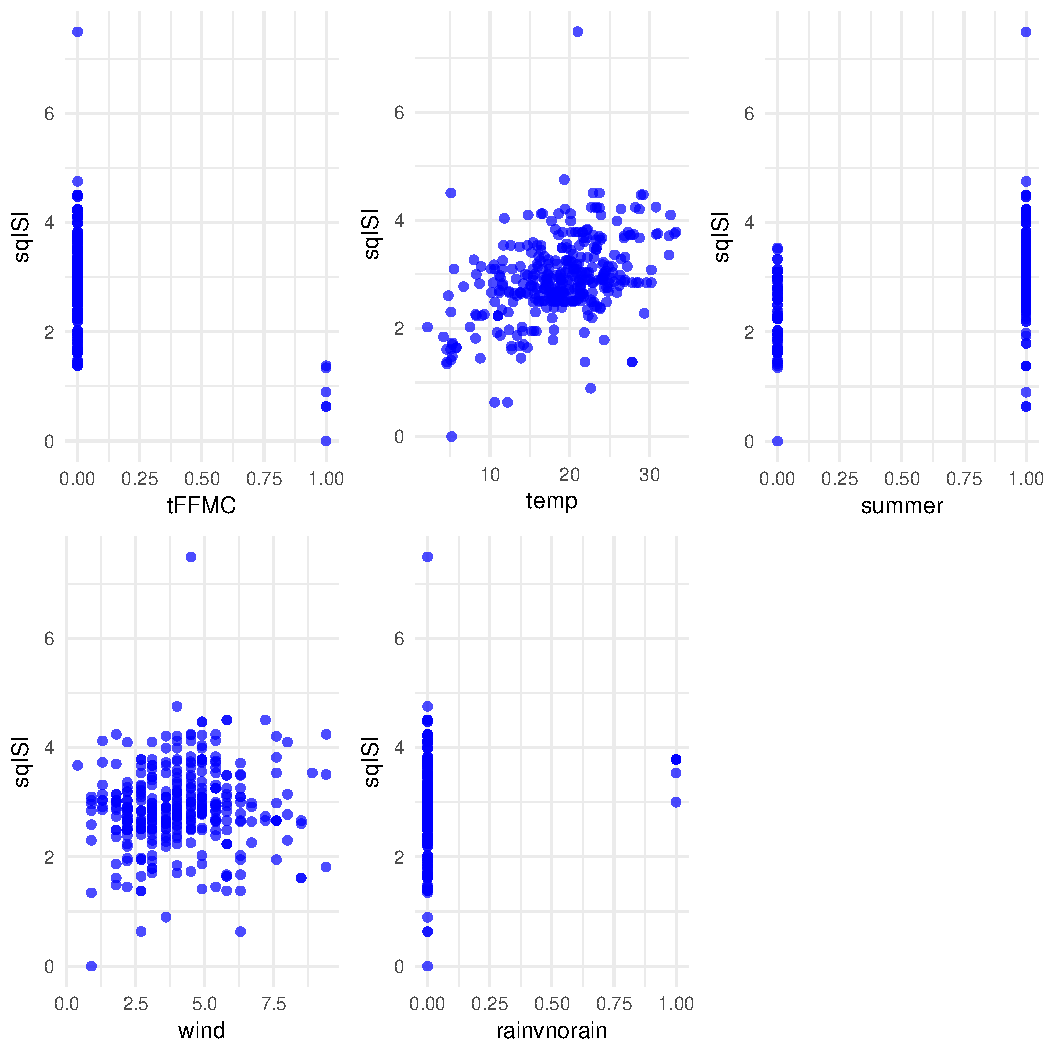
\includegraphics[width = .3\textwidth]{ISI_pairs.pdf}
}{%
  \caption{Bivariate plots of \textit{sqISI} and relevant covariates used in modeling}%
}
\end{floatrow}
\end{figure}
Using these coefficients values along with further investigation of added variable plots and initial model fits, we found that the variables \textit{wind}, \textit{summer}, \textit{temp}, \textit{tFFMC}, and \textit{rainvnorain} explain additional variance of \textit{sqISI}. A pairwise scatter plot can also be found in Figure 5. For this reason, we focus our modeling on these weather covariates along with the newly introduced variable \textit{tFFMC}. Seeing $tFFMC$ is the only non-weather covariate included, we attempt to use the information inherent in this variable in multiple ways which we discuss in the next section. 

\section{Modeling}
\subsection{Candidate Models}\label{candidate}
We consider models with \textit{rainvnorain}, \textit{temp}, \textit{summer}, and \textit{wind} as covariates.
%and include spatial coordinates, and use \textit{tFFMC} as a weight or random intercept.
Therefore, our primary mean function is given by 
\begin{equation}\label{mean_func}
\sqrt{ISI} = \beta_0 + \beta_1*Summer + \beta_2*Temperature + \beta_3*Rain + \beta_4 *Wind + e
\end{equation}
Upon fitting a regression model with this mean function, we found that the residuals appeared quite random, but were still not normally distributed. In an attempt to remedy this issue, we turned to weighted least squares models and mixed effects models with \textit{tFFMC} and several geo-spatial variables constructed in Section \ref{Engineering} as ways to account for the non-normal nature of the residuals.  
We fit a random intercepts model to each level in $grid\_group$ and to each coordinate group in $(X_2, Y_2)$. In both cases, we found no change in the distributions of the residuals. Moreover, we attempted weighting by the number of fires in each $grid\_group$ and each $(X_2, Y_2)$ block. Again, we saw no improvement in the behavior of the residuals.  We concluded that without further refinement or more granular data collection, all of the geo-spatial signal was being captured by the class of weather features, and therefore $X$, $Y$, and all derivative variables were excluded from our final model. 

Next, we consider $\textit{tFFMC}$ both as a weighting variable and as a covariate. By weighting points with $FFMC\leq 80$ differently, we inherently assume that these points have a different variance structure than the remaining data. Referring to Figure \ref{fig:FFMC_ISI_scatter}, we see that while this may be the case, with such few observations with $FFMC\leq 80$, any definitive conclusions about the variance structure are unjustified. However, assuming that this portion of the data is indeed different in some way than those with $FFMC > 80$, we fit a model with mean function given in \eqref{mean_func} plus $\textit{tFFMC}$, as well as a weighted least squares model with the weights corresponding to the number of observations for $\textit{tFFMC} = 0$ and $\textit{tFFMC} = 1$. Again, we see that the residuals maintain a similar random pattern, while the Q-Q plots change marginally, which is evident from Figure \ref{fig:ffmc_qq}. 
\begin{figure}[h!]
\centering
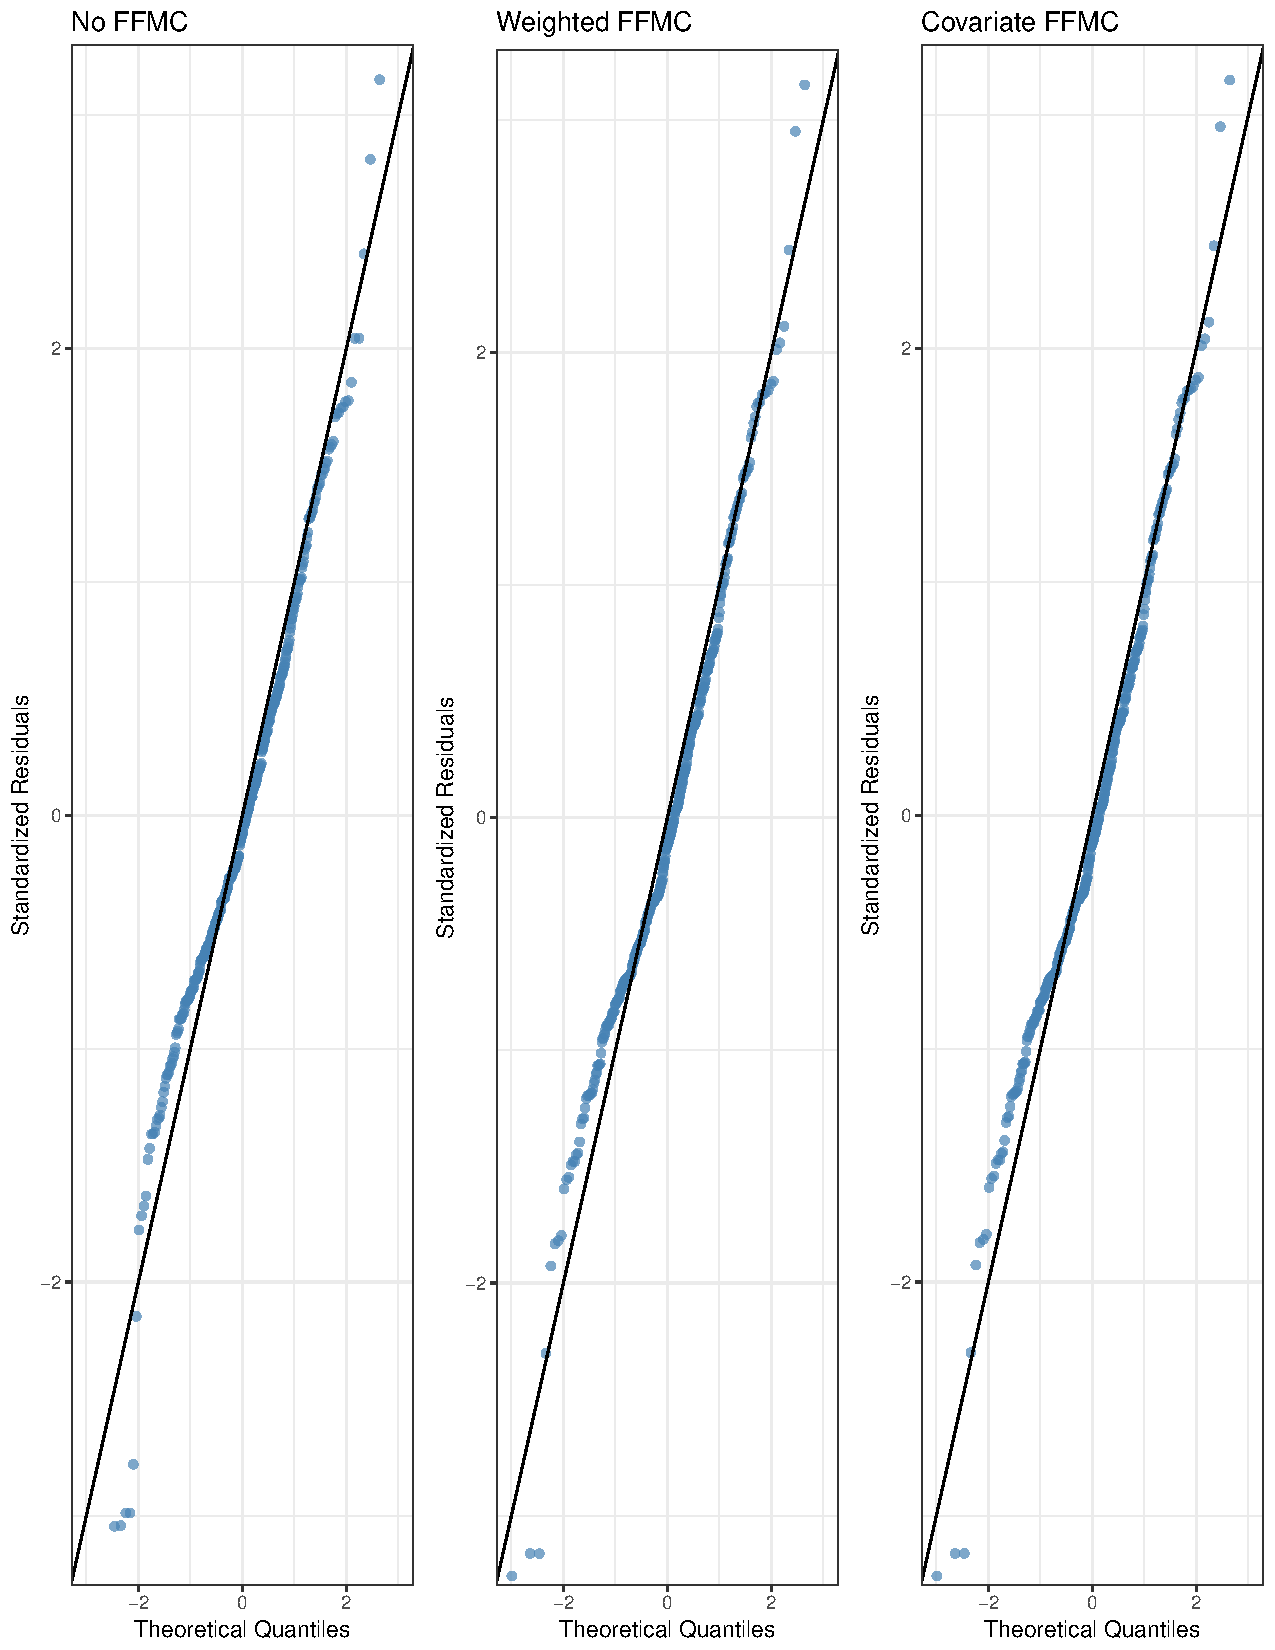
\includegraphics[width = .6\textwidth, height = 5cm]{FFMC-QQ.pdf}
\caption{The addition of \textit{FFMC} only marginally improves the linearity of residuals.}
\label{fig:ffmc_qq}{}
\end{figure}
Here, we scaled these plots to exclude the point where $ISI = 56.1$ (though it was used to train the models), as it skewed the graphics and hindered us from analyzing the normality assumptions of the standardized residuals. We note that there is still odd behavior at the tails of these distributions with the standardized residuals falling under and over the line $y = x$ at the theoretical quantiles greater than $\pm 1$. For this reason, we cannot justifiably use any model comparison techniques such as ANOVA. Instead, we note that the addition of $\textit{tFFMC}$ adds very little improvement to the normality of our errors when included as a covariate and as weights. Moreover, as we stated above, assuming that the points with $FFMC\leq 80$ have very different structure than those with $FFMC>80$ may be unreasonable based on this sample size. Therefore, for the sake of simple inferential statements, we do not include $\textit{tFFMC}$ in our final model.\footnote{As we stated in Section \ref{Background}, \textit{FFMC} relies on the weather covariates found in \eqref{mean_func}. Therefore, while we exclude $\textit{tFFMC}$ here, we implicitly include its effect via the remaining weather covariates.} The diagnostic plots of the final model described by \eqref{mean_func} can be found in Figure \ref{fig:fin_model}. 
\begin{figure}[h!]
\centering
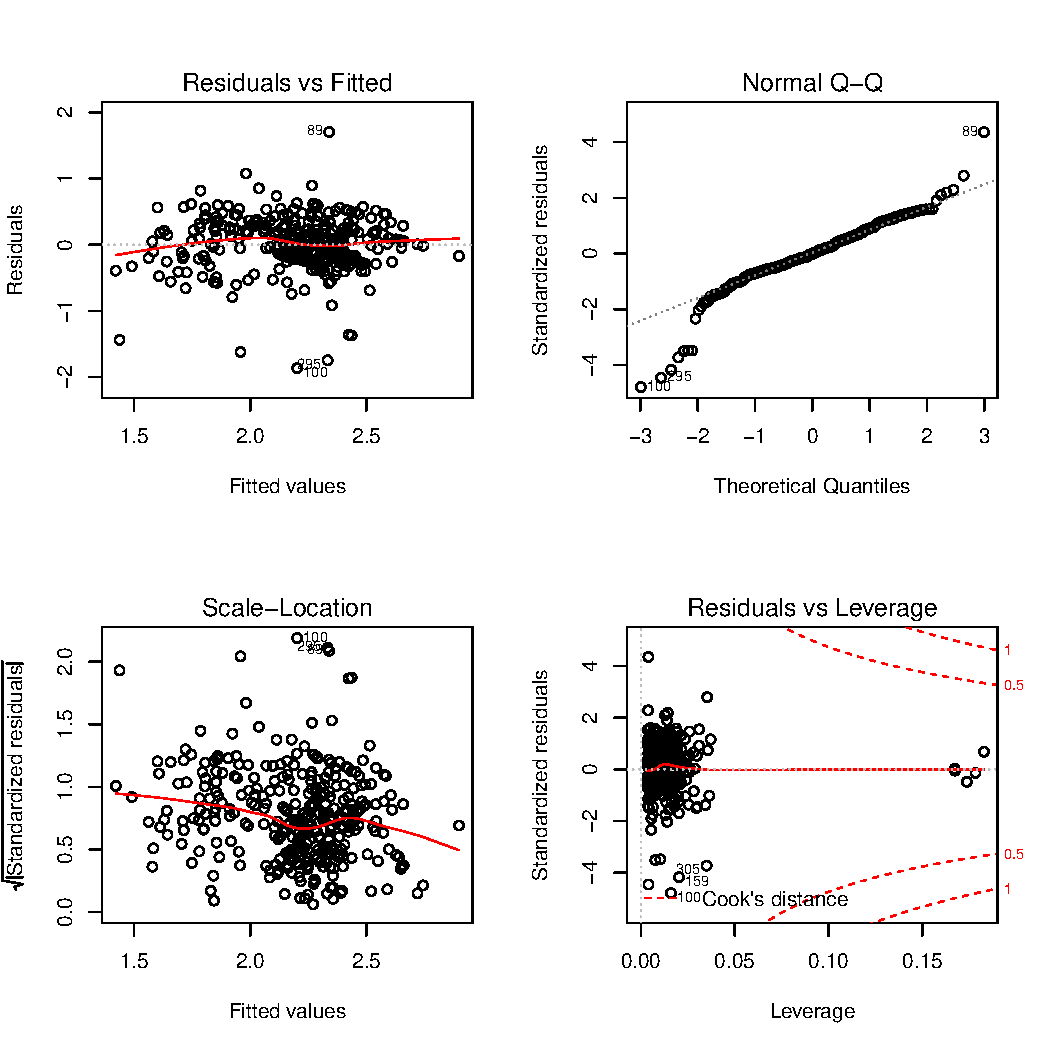
\includegraphics[width=.45\textwidth]{final_model_diag.pdf}
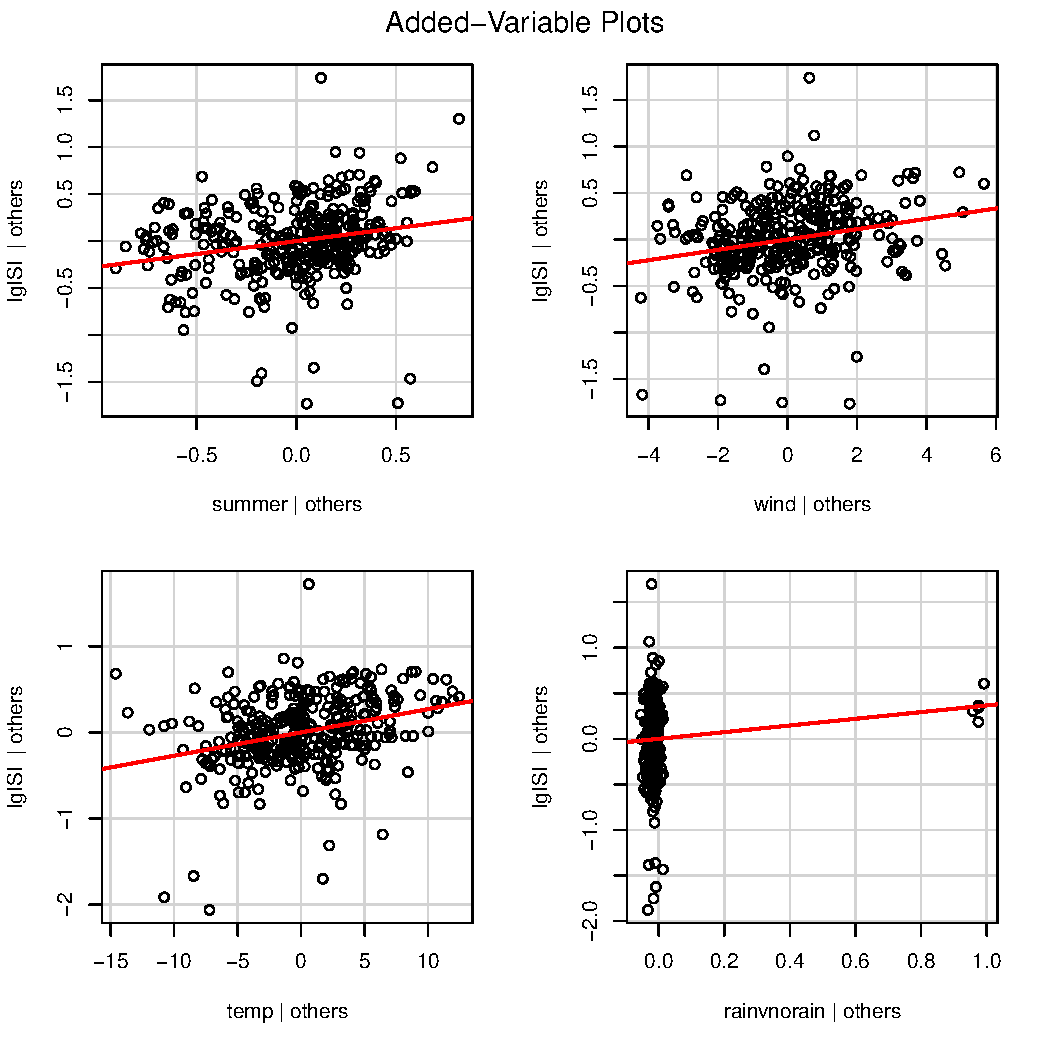
\includegraphics[width =.45\textwidth]{final_avp.pdf}
\caption{The final model appears to meet most modeling assumptions except that the residuals are normally distributed. The added variable plots suggest that each variable explains additional variance in \textit{sqISI}.}
\label{fig:fin_model}{}
\end{figure}
We note that the standardized residuals appear to be random noise around zero, with a few large outliers towards the center of the data. These points correspond to the outliers in \textit{ISI} but do not greatly affect the residual structure seen here. There appears to be a cluster of good leverage points as seen in the Residuals vs Leverage plot and we note that the Q-Q plot suggests that the residuals are not normal. Moreover, we see that the added variable plots suggest that each variable explains additional variance in the response $\textit{sqISI}$. Before we test for significance of these variables, we note that by having non-normal errors we cannot use classical theory suggesting that our estimates follow a $t$ distribution. Instead, we turn to a nonparametric technique to construct empirical confidence intervals (CI) for testing significance in our final model. 

\subsection{Bootstrapping}
Seeing that the residuals are non-normal in our final model, we instead use a nonparametric hypothesis testing framework to test the hypothesis $H_0: \beta_i = 0$ against $H_A:\beta_i \neq 0$. We implement the bootstrap procedure to construct sampling distributions of each $\beta_i$ and find the corresponding empirical CI. The results of this analysis are shown in Figure 8 and Table 2.
\begin{figure}[h!]
\begin{floatrow}
\ffigbox{%
  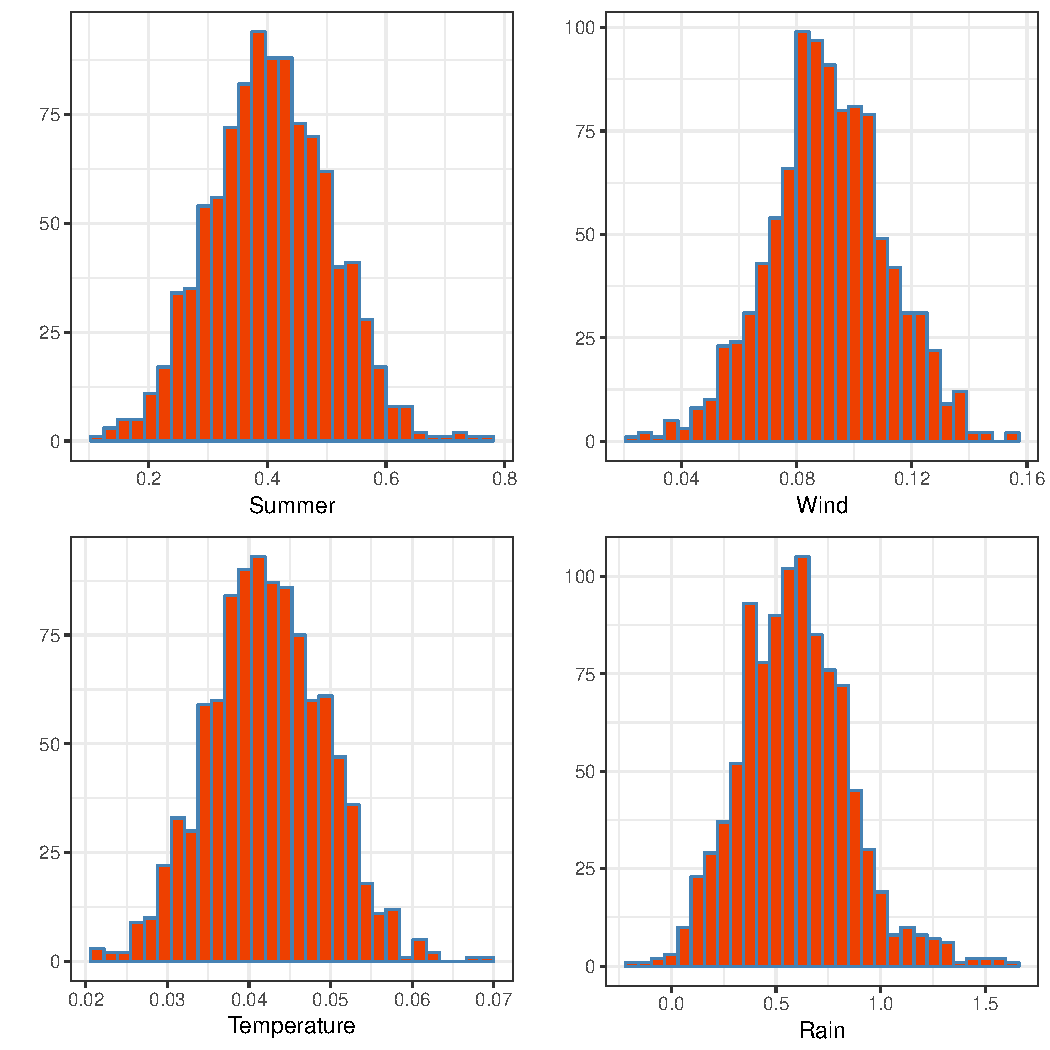
\includegraphics[width = .3\textwidth]{boot.pdf}
}{%
  \caption{Empirical sampling distributions of $\beta_i$}%
}
\capbtabbox{%
\begin{tabular}{|c|c|}\hline
Variable& 95\% Empirical CI\\
\hline
\hline
Wind & (0.06,\ 0.13)\\
Temperature & (0.03,\ 0.06)\\
Summer & (0.21,\ 0.61)\\
Rain & (0.11,\ 1.14)\\
\hline
\end{tabular}
}{%
  \caption{Empirical CIs}%
}
\end{floatrow}
\label{boot_res}
\end{figure}
We see that all sampling distributions are relatively normal and none of their confidence intervals contain $0$. This means that we can reject the null hypotheses and conclude that $\textit{summer},\textit{wind}, \textit{temp}$, and $\textit{rain}$ are all significant in explaining $\textit{sqISI}$.

\section{Prediction}\label{Prediction}

Finally, we turn our attention to evaluating the weather-only based model given by \eqref{mean_func} on the holdout set. We begin by fitting the chosen model on the testing data, which comprises 30\% of the original dataset. The results of this model are given in Figure \ref{fig:test_set_plots}. 
\begin{figure}[h!]
\centering
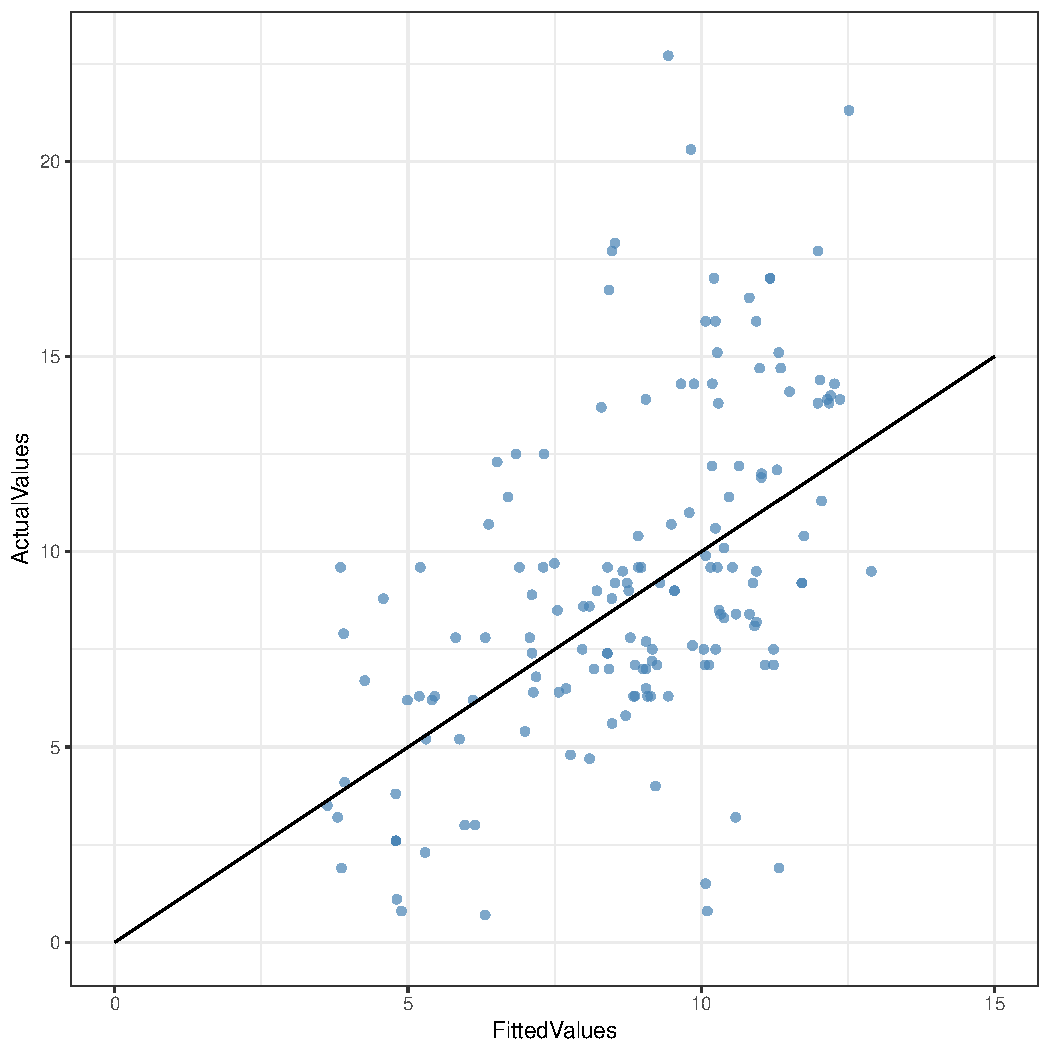
\includegraphics[width = .45\textwidth, height = 5.5cm]{pred_plot.pdf}
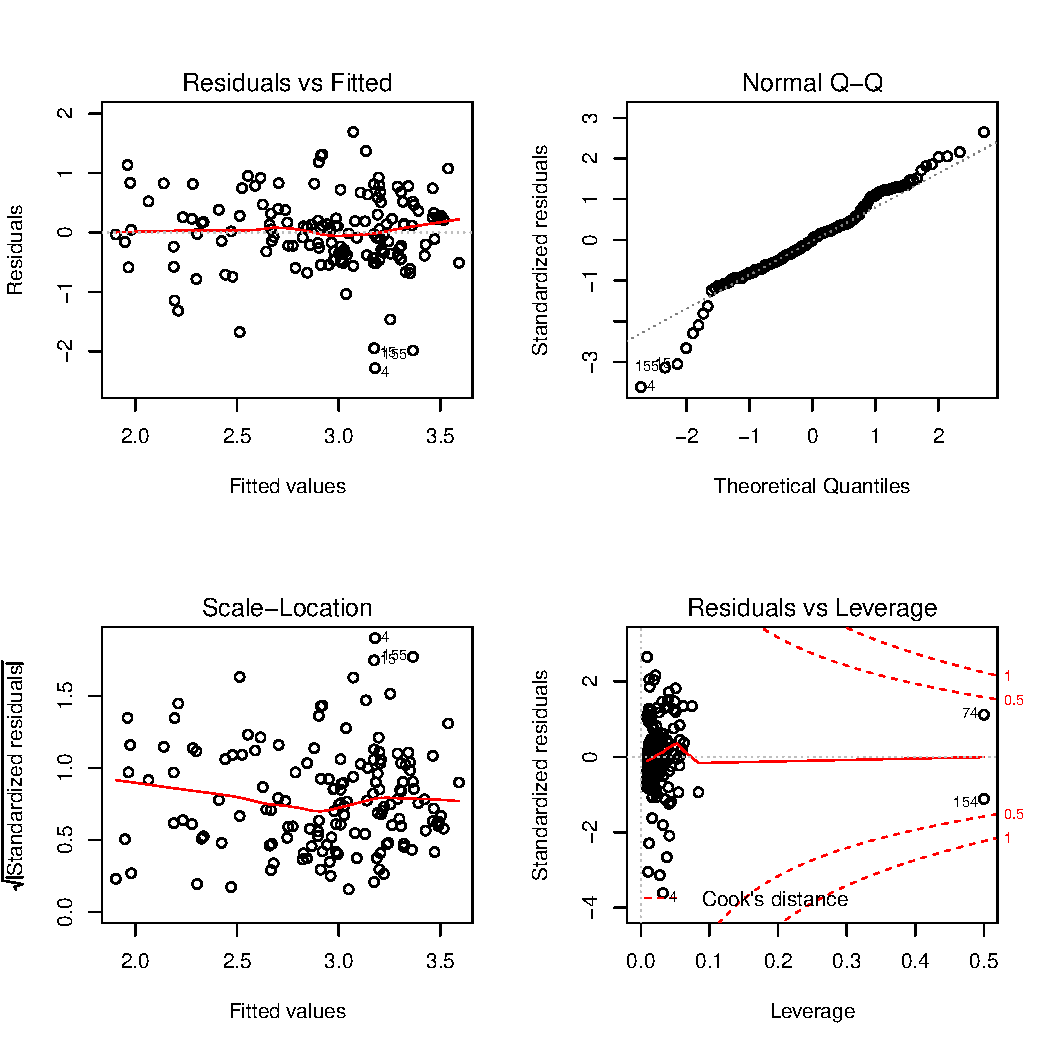
\includegraphics[width = .45\textwidth]{TestSetDiagnostics.pdf}
\caption{Testing results - predicted vs actual sqISI and model diagnostic plots.}
\label{fig:test_set_plots}
\end{figure}
In the Actual vs Predicted plot, we see that our inferential model captures the overall trend of \textit{sqISI}. Considering the predicted \textit{sqISI} values, the Mean Squared Error (MSE) was calculated to be $13.4$. In comparison, the MSE for the training set was $17.1$. However, as previously noted, there are significant outliers in the the training set, which explains the higher MSE.

Turning to the diagnostic plots in Figure \ref{fig:test_set_plots}, the model given here matches the behavior of the model fit on the training data. That is, our residuals appear random yet non-normal. This can be seen in the $Q-Q$ plot, which exhibits significant left tail behavior. Therefore, CIs for our coefficient estimates were constructed from a bootstrap sample. We then use these to make conclusions about the significance of the covariates. The results of this analysis are summarized in Table 3 and Table 4. 
%table numbers hard coded! if we add anything change this! 

\begin{table}[h!]
\begin{floatrow}
\capbtabbox{%
\begin{tabular}{ | l | c | c |}\hline
  Variable & Estimate & Standard Error \\ \hline
  Intercept & 1.31 & 0.24 \\
  Is Summer & 0.58 & 0.16 \\
  Wind & 0.079 & 0.029 \\
  Temperature & 0.045 & 0.012 \\
  Is Raining & -0.26 &   0.47 \\
  \hline
\end{tabular}\label{test_coef}
}{%
  \caption{Coefficient estimates on testing set}%
}
\capbtabbox{%
	\begin{tabular}{  | l | c | }\hline
  Variable & $95\%$  CI \\ \hline
  Intercept & $(  0.86,\ 1.76 )$ \\
  Is Summer & $( 0.27,\ 0.91)$\\
  Wind & $(0.02,\ 0.13  )$ \\
  Temperature & $(0.02,\ 0.07)$ \\
  Is Raining & $(-1.30,\ 0.59)$ \\
  \hline
\end{tabular}
}{%
  \caption{Test set empirical CIs}%
}
\end{floatrow}
\end{table}
All the CIs except for the binary \textit{Is Raining} variable in Table 4 do not contain zero, so we conclude that they are all different than zero. As the \textit{Is Raining} CI does contain zero, we do not conclude that the \textit{Is Raining} variable is significantly different than zero. We also note that the CI is quite wide and there is a large standard error, because there were only two data points with rain in the test set. While rain was uncommon in the training set, it was less sparse than in the testing set, so it is difficult to make inferences on such a variable. 

The analysis on the testing set mostly confirms the model selection performed on the training set, with the key difference being the loss of significance for the \textit{Is Raining} variable.  We conclude that all weather variables except for \textit{rain} impact \textit{sqISI}, and fail to conclude that the presence of rain is a predictor for the model. Based on an MSE criterion, the predictions from the model are reasonably close to the actual data.

\section{Discussion}\label{Discussion}

%For the goals of Cortez and Morais, every data point representing an individual fire is sufficient. However, for our goal of predicting \textit{ISI}, if we only look at data where fires occurred, then our predictions will not necessarily generalize to other data. Our intended use case is prior to the knowledge of whether there is or is not a fire. Yet, all the data is sampled from a posterior distribution given that a fire occurred.

%Furthermore, consider the situation where the models outlined in this paper were used to influence where to pre-burn the brush, or otherwise reduce \textit{ISI}. Then the new data points are sampled from unburnt areas, and thus a different distribution as our training data. Thus, a comprehensive data set would be preferred; ideally measurements being recorded every day for some period. 

After a thorough modeling process, we selected the variables \textit{Wind}, \textit{Temperature}, \textit{Summer}, and \textit{Rain} based on a LASSO-driven approach to variable selection. Higher wind speeds, high temperatures, and summertime conditions all correspond to higher \textit{ISI} while the presence of rain did not play a role in predicting \textit{ISI}. 
%Other variables related to the moisture content characterizing contents of deeper soil layers were deemed insignificant for predicting the \textit{ISI}, with the exception of \textit{FFMC}. Therefore, when predicting the impact on initial spread, we only considered surface layer conditions of the forest. 
Wind was found to be the most important predictor of \textit{ISI}, so when considering fire conditions, predicting wind speed and allocating resources based on this quantity should be prioritized. In addition, warm temperatures are an important consideration when predicting fires. Summertime was also predictive of \textit{ISI}, which we suggest captures other underlying weather features such as long stretches of dry weather that are not otherwise captured in the data. These findings match our intuition that dry, windy conditions are conducive to rapid fire spread. 

As noted throughout this report, there is a latent observation bias throughout our dataset: each of the observations represents a single fire. As a result, our observations are imbalanced across spatial coordinates, months of year, and even days of the week despite the fact that \textit{ISI} is defined, though not recorded, even when no fire occurs. Therefore, to conduct a complete analysis, one must collect data relating the covariates considered here and \textit{ISI} uniformly over the course of time with disregard to the presence of a fire. This will remove any implicit effect that fires have on \textit{ISI} as well as the human effect discussed throughout the duration of this report. By collecting temporal and spatial data, the effect of weather and topographical attributes may be tested directly.  

Throughout our report, we focus primarily on an inferential approach. That is, we only consider simple, interpretable models that provide insight to the \textit{ISI} and, by extension, determine what causes initial rapid spread of fires. In this way, we sacrifice predictive accuracy, because as previously noted, \textit{FFMC} is highly non-linearly predictive, and thus if we simply wanted to predict \textit{ISI}, we could build a complex function of \textit{FFMC} to predict \textit{ISI}, at the cost of interpretability of the model. We choose to keep the interpretable model, because the loss of predictive power is minimal and we prefer to investigate the direct cause of weather impacts on the initial spread of fire. Moreover, this approach empowers firefighting organizations to focus on real-time, easily accessible data when allocating resources to stop fires at their source.   

Based on these results, we suggest further investigation into the impact of summer conditions on \textit{ISI}, and the impact of a the Portuguese Mediterranean climate. In particular, focus could be on the specific climatic differences during the summertime and the impact on fire susceptibility in ways that are not captured by other indicies such as \textit{DC} or \textit{DMC}. Similarly, Portuguese forestry officials could measure changes in the forest through the year including the amount of dry grass on the forest floor and other flammable vegetation to gather additional data to predict the initial spread of fires.

\end{document}